
\chapter{1st class -- problem definition}

\section{Our equation}

Many problems in engineering practice can be described by 
\begin{equation}
\label{oureq}
 - (p u')' + q u = f,
\end{equation}
 where $u$ is the solution, $p$ and $q$ are coefficients, $f$ is a scalar function.  It is known that solution of \eqref{oureq} 1) exist and 2) is unique, if $p > 0$ for the given boundary conditions
 \begin{equation}
 \label{dirbc}
  \begin{split}
   u(0) &= u_{0}, \\
    u(1) & = u_{1},
  \end{split} 
 \end{equation}
or 
\begin{equation}
\label{dirneubc}
 \begin{split}
      u(0) &= u_{0}, \\
    u'(1) & = \vec{q}_{1},
 \end{split} 
\end{equation}
or 
\begin{equation}
\label{robinbc}
 \begin{split}
  \alpha_{0}u(0) + \alpha_{1}u'(0) &= a ,\\
     \beta_{0}u(1) + \beta_{1}u'(1) &= b ,
 \end{split} 
\end{equation}
where \eqref{dirbc} is a combination of Dirichlet conditions, \eqref{dirneubc} is a combination of Dirichlet and Neumann conditions, and \eqref{robinbc} is a combination of mixed (Robin) conditions.

For more spatial dimensions \eqref{oureq} is formulated as
\begin{equation}
\label{oureqD}
- \nabla \cdot (\mathbf{P} \nabla u)  + qu = f .
\end{equation}

\section{Approximate solution}
Since exact solution is often unknown, as direct integration is in 
many real world cases  impossible, an approximate solution to \eqref{oureq} or \eqref{oureqD} can be constructed out of polynomials and so
\begin{equation}
\label{bencheq}
 u \approx p_{n}(x) = \sum_{i=0}^{n}\pi_{i} x^{i} 
\end{equation}


if $n = 1$ then coefficients $\pi_{0,1}$ can be simply obtained from boundary conditions and so
\begin{equation}
 \begin{split}
  u_{0} &= p_{1}(0) = \pi_{0}, \\
   u_{1} &= p_{1}(1) = \pi_{1},
 \end{split} 
\end{equation}
it is apparent, that definition of $\pi_{0,1}$ satisfying the given Dirichlet conditions has no relation to our equation!

Let us assume the following benchmark example
\begin{equation}
\label{benchsin}
 -u'' + 4u  = \sin 3x.
 \end{equation}
It is known that the exact solution is  
\begin{equation}
u(x) = \alpha \exp(2x) + \beta \exp(-2x)+ \frac{1}{13} \sin 3x,  
\end{equation}
where $\alpha$ and $\beta$ are defined by boundary conditions setup. If 
we set $\alpha = 0$ and $\beta = 1$, then the boundary conditions state 
that
\begin{equation}
\begin{split}
  u(0) &= 1, \\
  u(1) &= \exp(-2) + \frac{\sin 3}{13}
\end{split}
\end{equation}

With increasing value of $n$ we can define a well known method for approximating differential equations -- {\it collocation method}.

The method can be demonstrated as follows.

For polynomial approximation of degree $n=1$, solution is 
approximated by \begin{equation}p_{1}(x) = \pi_{1}x + \pi_{0}\end{equation}, and so $\pi_{0}=1$. 
The coefficient $\pi_{1}$ is obtained from the second boundary 
condition and so
\begin{equation}
\begin{split}
 p(1)_{1} = \pi_{1}\times 1.0 + \pi_{0} = \exp(-2) + \frac{\sin 3}{13} 
 \Rightarrow \pi_{1} = \exp(-2) + \frac{\sin 3}{13}  - 1.
 \end{split}
\end{equation}
It is apparent that definition of $\pi_{0,1}$ had no relation to 
\eqref{benchsin}. And so we shoudl search for higher degree 
approximation.

If $n=2$, then 
\begin{equation}p_{2}(x) = \pi_{2}x^{2} +\pi_{1}x + \pi_{0}\end{equation},
then let's select some interior point for which the equation 
\eqref{benchsin} is 
satisfied, eg. $x_{int}=0.5$.

Then we can constitute the following system of linear equations for 
$\pi_{0,1,2}$.

\begin{equation}
 \label{systemcolloc} 
 \begin{split}
  \pi_{0} &= 1 \qquad \mbox{ \fs (1st boundary condition)} \\
  \pi_{0} + \pi_{1} \times 1.0 + \pi_{2} \times 1.0^{2} &=  \exp(-2) + 
  \frac{\sin 3}{13} \qquad  \mbox{ \fs (2nd boundary condition)} \\
  \pi_{0} + \pi_{1}\times 0.5 + \pi_{2} \times 0.5^{2} &= \sin (3 
  \times 0.5) \qquad \mbox{ \fs (interior point)}.
 \end{split} 
\end{equation}
Analogicaly for $n=3$, approximation polynomial is then
\begin{equation}p_{3}(x) = \pi_{3}x^{3} + \pi_{2}x^{2} +\pi_{1}x + 
\pi_{0},\end{equation} interior points will be then
$x_{int_{1}}=\sfrac{1}{3}$ , and $x_{int_{2}}=\sfrac{2}{3}$. Similar 
system to \eqref{systemcolloc} is then assembled. Convergence of the 
collocation method for the selected benchmark problem is apparent from 
figure~\ref{collocconv}.
\begin{figure}
\centering
 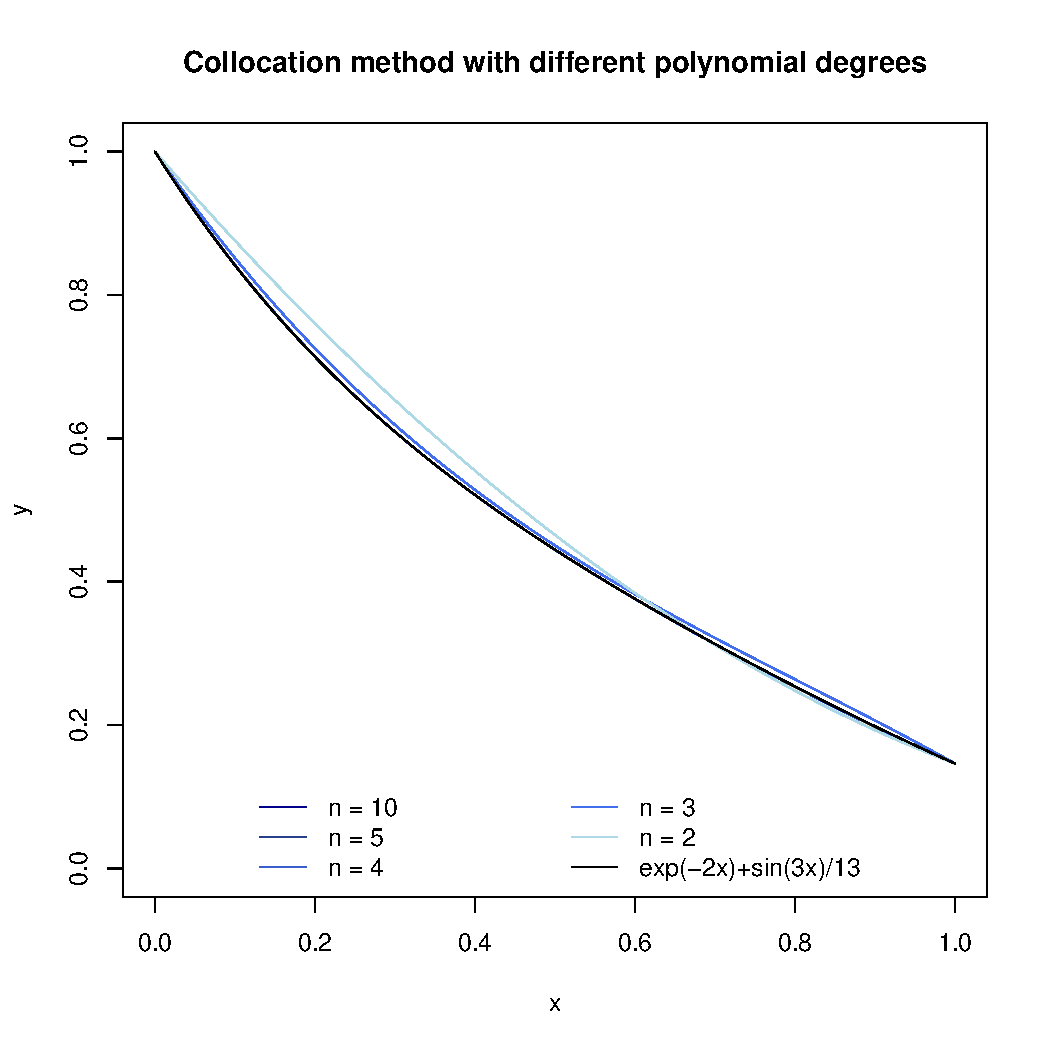
\includegraphics[width=9cm]{images1/collocation_adv_numerics.pdf}
 \label{collocconv}
 \caption{Approximating benchmark problem \eqref{benchsin} with 
 polynomials constructed with collocation method.}
\end{figure}

The collocation method is an analogy to Lagrangian interpolation with the same quality properties  -- possibly divergent prone!!. A disputable approach, error is measured at discrete points, but we are searching for a continuous approximation!.


Another approach for defining the error continuously is {\it least square method} (later it will be defined as {\it least-square-finite-element-method} (here after LSFEM).

In order to simplify our notations our problem \eqref{oureq} will be expressed in terms on differential operator
\begin{equation}
%\label{oureq}
 \overbrace{- (p u')' + q u = f}^{Lu}.
\end{equation}
let $u_{h}$ be the approximation of $u$. The LSFEM method measures approximation error as
\begin{equation}
 \varepsilon = \int\limits_{\Omega} (L u_{h} - f )^{2} \dd \Omega,
\end{equation}
and so the solution is obtained by setting
\begin{equation}
  \int\limits_{\Omega} (L u_{h} - f )^{2} \dd \Omega \leadsto \mbox{min}.
\end{equation}

And so \eqref{bencheq} if $\alpha=0$ and $\beta=1$ can be solved as 
\begin{equation}
 \int\limits_{0}^{1} (  -u'' + 4u  - \sin 3x )^{2} \dd x \leadsto \mbox{min} \wedge p(0) = 1 \, \& \, p(1) = \exp(-2) + \sin\left(\frac{3}{13}\right),
\end{equation}
which is just a constraint minimization.

Another approach is 
\begin{equation}
 \int\limits_{0}^{1} (  -u'' + 4u  - \sin 3x )^{2} \dd x  + P_{0} (p_{n}(0)-u_{0})^{2} + P_{1} (p_{n}(1) - u_{1})^{2}\leadsto \mbox{min} ,
 \end{equation}
where $P_{0,1}$ are penalization constants, by setting $P_{0,1}$ values we define how important satisfying the boundary conditions is, theoretically if $P_{0,1} \leadsto \infty$ the boundary conditions are exactly satisfied, however, our solution became independent on the governing equation.

The bottle neck of these methods is that it is difficult to relate these residuals to physical properties. And so yet another approach will be defined here. Let's define scalar product and our operator $L$ as
\begin{equation}
\begin{split}
 (L(u),v) &= (v, L(u)) \\
  L(u + v) &= L(u) + L(v) \\
  L(\alpha u) &= \alpha L(u) \\
  (L(u),v) &\ge c(u,v), \; \exists c>0.
\end{split}
\end{equation}
The last condition implies that our operator is {\it positive definite}.

Then let us define 
\begin{equation}
 E(u) = (L(u),v) - 2(f,v),
 \end{equation}
 where $E$ is energy functional -- an energy of our system. There is a proof, which says that minimizing $E$ leads to a best approximation of our solution. Such method is referred to as Ritz method. 
 
 Problem with using just polynomials starts with more dimensions. It is still relatively simple to find polynomial satisfying given boundary conditions for rectangular.
 
 \begin{center}
 \begin{tikzpicture}
\draw [draw=black] (3.0,3.0) rectangle (0.3,0.3);
%\filldraw [fill=Peach, draw=black] (11.1,5) rectangle (0.3,0.3);
%\filldraw [fill=RedOrange, draw=black] (11.1,4.5) rectangle (0.3,0.3);
\end{tikzpicture}
\end{center}
 
 
 \begin{equation}
  -\Delta u = 1 , \; \Omega = (0,1) \times (0,1), \; \restr{u}{\Gamma} = 0, 
 \end{equation}
 which is 
 \begin{equation}
  u_{h} = x(1-x)(1-y) \sum_{i}^{n} \sum_{i}^{n}\pi_{i,j}x^{i}y^{i}. 
 \end{equation}
 
 
 But issues start with L-shape $\Omega = (0,1) \times (0,1) - (\sfrac{1}{2},1) \times (\sfrac{1}{2},1) $

 
 \begin{center}
 \rotatebox{0}{
 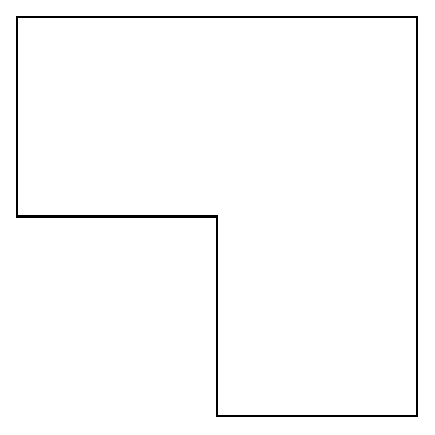
\includegraphics[width=4cm]{images1/lshape.eps}}
 \end{center}

 It is impossible to find polynomial, which satisfies the given boundary conditions.
 

 
